\documentclass{article}

\usepackage[utf8]{inputenc}
\usepackage{amsmath}
\usepackage{booktabs}
\usepackage{graphicx}
\usepackage{float}
\usepackage[margin=1in]{geometry}
\setlength{\parindent}{0pt}
\setlength{\parskip}{0.5em}

\title{Comparing Recommender System Architectures}
\author{Aman Krishna Uppuluri}
\date{}

\begin{document}

\maketitle

\section{Introduction}

In this report, three recommender system architectures based on collaborative filtering were implemented and compared:

\begin{itemize}
    \item Matrix Factorization (MF)
    \item MLP-based Neural Collaborative Filtering (MLP)
    \item NeuMF (Neural Matrix Factorization)
\end{itemize}

The models were evaluated using Hit@10 under two negative sampling strategies:

\begin{itemize}
    \item Uniform negative sampling
    \item Popularity-based weighted negative sampling
\end{itemize}

The goal was to study how model architecture, embedding dimension, and negative sampling strategy affect recommendation performance.

\section{Approach}

MF models user-item interactions using a dot product between user and item embeddings:

\[
\hat{y}_{ui} = \mathbf{p}_u^T \mathbf{q}_i
\]

MLP-based collaborative filtering instead concatenates user and item embeddings and learns a non-linear interaction function through fully connected layers.

\[
\hat{y}_{ui} = f(\mathbf{p}_u, \mathbf{q}_i \mid \theta)
\]

NeuMF combines both approaches: it runs a GMF path and an MLP path in parallel, then merges their outputs.

\[
\hat{y}_{ui} = \sigma \left( \mathbf{h}^T 
\begin{bmatrix}
\mathbf{p}_u \odot \mathbf{q}_i \\
f(\mathbf{p}_u, \mathbf{q}_i)
\end{bmatrix}
\right)
\]

\subsection{Geometric Interpretation of MF vs MLP}

Matrix Factorization (MF) assumes that users and items can be represented as points in a single latent geometric space. The interaction score is determined by the geometric relationship between these vectors, ie. dot product. This means that similar users and items must be placed close together in the latent space.

However, the latent space is shaped entirely by the training data. Since all user and item vectors are constrained simultaneously by many observed interactions, the model must find a compromise arrangement that satisfies as many relationships as possible. Even with higher embedding dimensions, some interaction constraints may still be impossible to represent perfectly.

MLP-based recommenders do not rely on geometric similarity in a fixed latent space. Instead, they learn a non-linear interaction function over the concatenated user and item embeddings. Because the interaction function is learned directly from data rather than enforced geometrically, MLP models are more flexible and can learn more complex interaction patterns that MF may struggle to represent.

\section{Experimental Setup}

Negative sampling was performed dynamically every epoch. In addition to standard uniform negative sampling, popularity-based weighted negative sampling was implemented using weighted random sampling (WRS). This produced harder negative examples by sampling popular items more frequently. Harder negative examples are examples which the user has not interacted with, that are still highly reasonable recommendations for them, making them harder for the model to distinguish from true positive interactions. They are simply negatives which seem like positives.


\begin{itemize}
    \item Embedding dimensions tested: 8, 16, 32, 64
    \item Epochs: 25
    \item Evaluation metric: Hit@10
    \item Optimizer: Adam
    \item Loss function: Binary Cross Entropy Loss
\end{itemize}

As embedding dimension increased, the differences between the architectures became significantly more pronounced. In particular, NeuMF began to substantially outperform both MF and MLP at larger embedding dimensions under weighted negative sampling. Therefore, much of the later analysis focuses on the case of $embedding\ dimension = 64$, where the differences are most visible.



\section{Results and Analysis}

\subsubsection*{Uniform Negative Sampling}

\begin{center}
\begin{tabular}{ccccc}
\toprule
Embedding Dimension & MF & MLP & NeuMF \\
\midrule
8  & 0.5246 & 0.5197 & 0.5130 \\
16 & 0.5423 & 0.5536 & 0.5325 \\
32 & 0.5057 & 0.5783 & 0.5079 \\
64 & 0.4241 & 0.5696 & 0.5250 \\
\bottomrule
\end{tabular}
\end{center}

\vspace{0.5cm}

\subsubsection*{Weighted Negative Sampling}

\begin{center}
\begin{tabular}{ccccc}
\toprule
Embedding Dimension & MF & MLP & NeuMF \\
\midrule
8  & 0.2983 & 0.4025 & 0.4684 \\
16 & 0.3791 & 0.4398 & 0.5130 \\
32 & 0.3941 & 0.5101 & 0.6144 \\
64 & 0.4123 & 0.5980 & 0.7849 \\
\bottomrule
\end{tabular}
\end{center}
\subsection{Final Results}

\subsubsection*{For Embedding Dimension 64}
\begin{center}
\begin{tabular}{cccc}
\toprule
Model & Sampling & Hit@10 \\
\midrule
MF & Uniform & 0.4241 \\
MLP & Uniform & 0.5696 \\
NeuMF & Uniform & 0.5250 \\
MF & Weighted & 0.4123 \\
MLP & Weighted & 0.5980 \\
NeuMF & Weighted & 0.7849 \\
\bottomrule
\end{tabular}
\end{center}

Figure~\ref{fig:embdim} shows the effect of embedding dimension on recommendation performance for all models under both sampling strategies.

\begin{figure}[H]
\centering
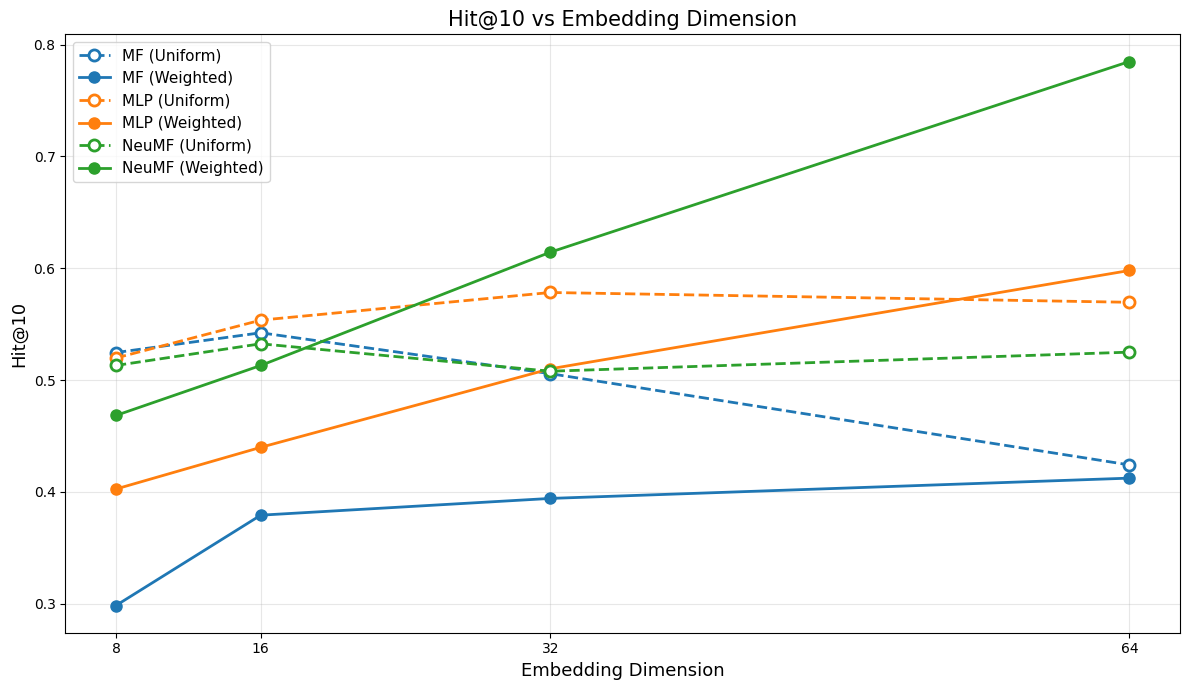
\includegraphics[width=0.92\textwidth]{score vs emb_dim.png}
\caption{Hit@10 versus embedding dimension for MF, MLP, and NeuMF under uniform and weighted negative sampling.}
\label{fig:embdim}
\end{figure}

Several important trends can be observed:

\begin{itemize}
    \item MLP consistently outperformed MF under uniform sampling.
    \item NeuMF barely showed only gains under uniform sampling.
    \item Under weighted sampling, NeuMF performance increased dramatically as embedding dimension increased.
    \item MF benefited the least from larger embedding dimensions.
\end{itemize}

\subsection{Training Performance at Embedding Dimension 64}

The following figures analyze model behavior at $embedding\ dimension = 64$, where the differences between the architectures were most pronounced.

\begin{figure}[H]
\centering
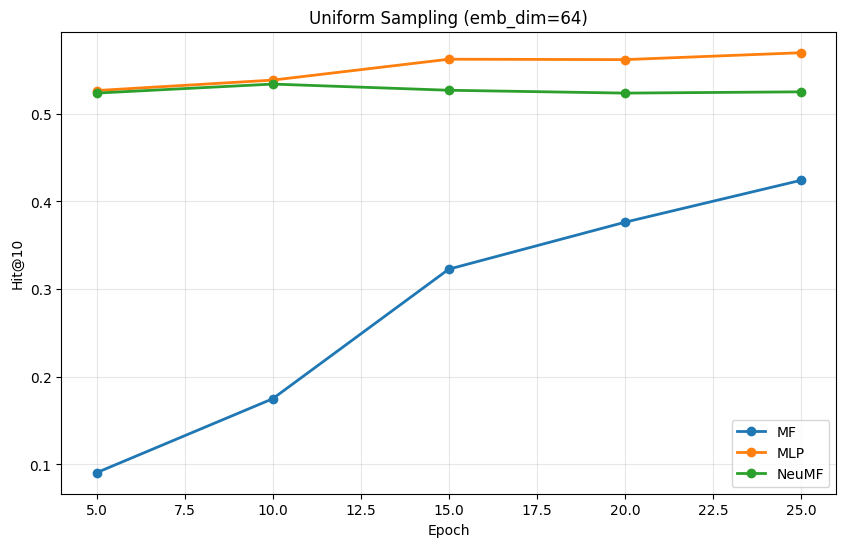
\includegraphics[width=0.82\textwidth]{uniform sampling (64).png}
\caption{Hit@10 versus epochs under uniform negative sampling for embedding dimension 64.}
\label{fig:uniform64}
\end{figure}

Under uniform sampling, MLP achieved the best performance while NeuMF provided only limited improvement. One possible reason is that uniformly sampled negatives are relatively easier to distinguish, reducing the advantage provided by NeuMF’s more expressive interaction modeling. Slight overfitting was also observed for NeuMF.

\begin{figure}[H]
\centering
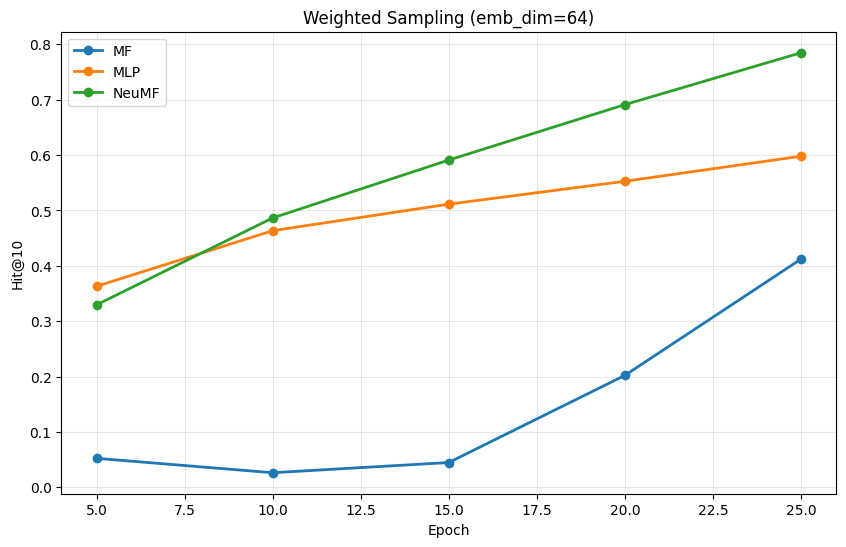
\includegraphics[width=0.82\textwidth]{weighted sampling (64).png}
\caption{Hit@10 versus epochs under weighted negative sampling for embedding dimension 64.}
\label{fig:weighted64}
\end{figure}

Under weighted sampling, NeuMF dramatically outperformed both MF and MLP. As training progressed, the performance gap widened, suggesting that neural models benefit more from difficult negative examples. 

\begin{figure}[H]
\centering
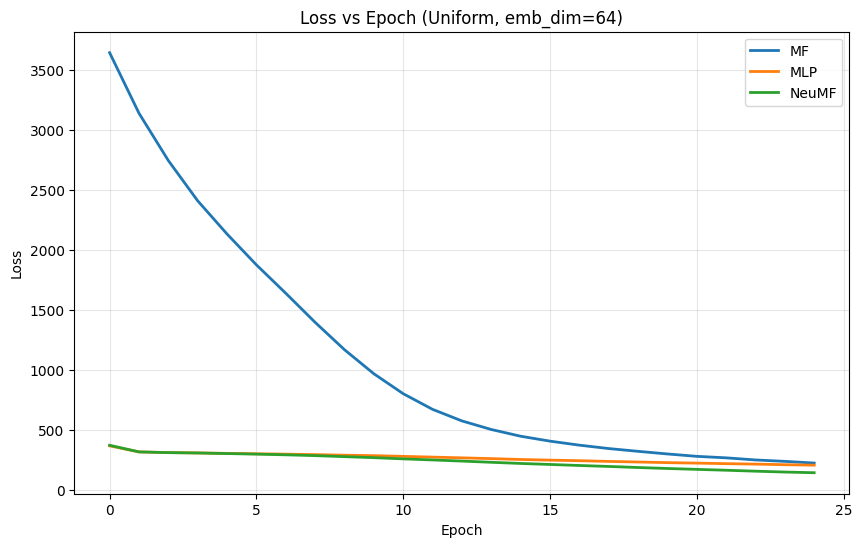
\includegraphics[width=0.82\textwidth]{loss vs epoch uniform 64).png}
\caption{Training loss versus epochs under uniform sampling for embedding dimension 64.}
\label{fig:lossuniform}
\end{figure}

The loss curves under uniform sampling indicate relatively stable convergence behavior. However, despite decreasing loss, NeuMF did not significantly improve ranking performance, suggesting that the model complexity exceeded the difficulty of the training signal.

\begin{figure}[H]
\centering
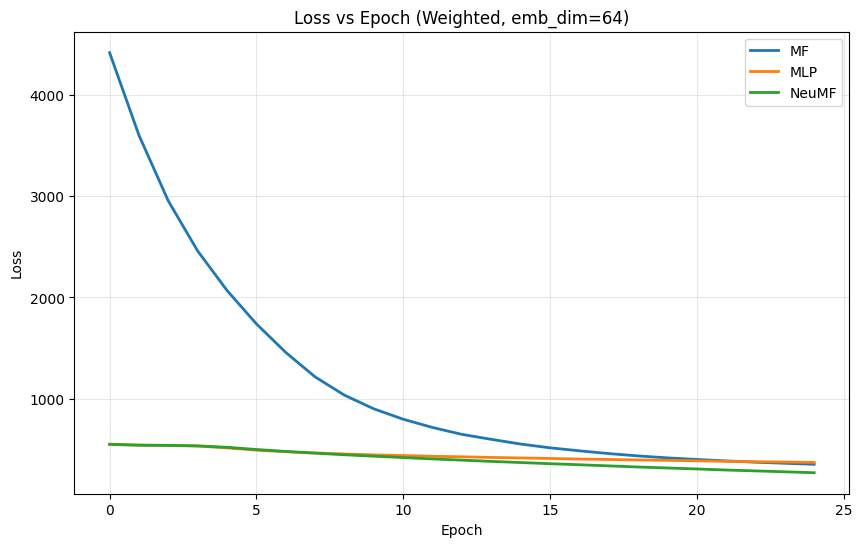
\includegraphics[width=0.82\textwidth]{loss vs epoch weighted 64).png}
\caption{Training loss versus epochs under weighted sampling for embedding dimension 64.}
\label{fig:lossweighted}
\end{figure}

Under weighted sampling, NeuMF achieved both lower training loss and substantially higher Hit@10 performance. This indicates that harder negative examples allowed the model to better utilize its expressive capacity.

\subsection{Effect of Large Embedding Dimensions}

During experimentation, NeuMF was tested with an embedding dimension of 128 
combined with weighted sampling. The results were 
striking — Hit@10 reached 0.98 by epoch 25, far exceeding any result 
observed at smaller embedding dimensions.

This suggests that NeuMF benefits greatly from larger embedding 
capacity when paired with smarter negative sampling. A larger embedding 
dimension allows the GMF and MLP pathways to capture richer latent 
structure, while weighted negative sampling provides harder, more informative negatives that 
push the model to learn finer distinctions between relevant 
and irrelevant items.

\section{Key Observations}

\begin{itemize}
    \item MF performed reasonably well on easier uniform negatives but struggled under weighted sampling.
    
    \item MLP consistently benefited from larger embedding dimensions because of its ability to model non-linear user-item interactions.
    
    \item NeuMF only showed major gains when both embedding dimension and negative difficulty increased.
    
    \item Weighted negative sampling proved effective for neural recommenders.
    
    \item The combination of linear and non-linear interaction modeling in NeuMF produced the strongest overall performance.
\end{itemize}

\section{Conclusion}

The experiments demonstrated that both model architecture and negative sampling strategy strongly influence recommendation performance.

NeuMF achieved the best overall performance, especially under weighted negative sampling and larger embedding dimensions. Also, MLP consistently outperformed MF, while MF struggled to model accurately.


\section{Answers to Questions in Notebook}

\begin{enumerate}

\item \textbf{Why are we sampling negatives only for the training data?}

Negative sampling is required during training because the model must learn from both positive and negative examples. During testing, there is no learning of the model.

\item \textbf{Why might the MLP model outperform MF?}

MLP can learn complex non-linear user-item interactions, whereas MF is limited to linear dot-product interactions. This makes MLP more capable of capturing deeper patterns.

\item \textbf{In what cases might MF perform just as well or better?}

MF can perform well when the user-item interactions are relatively simple. It is also computationally faster and less prone to overfitting as compared to MLP.

\item \textbf{How does embedding size affect performance?}

Larger embedding dimensions generally improved the performance of neural models, especially NeuMF under weighted negative sampling, because larger latent spaces can capture deeper interaction patterns.

\item \textbf{Did you observe any signs of overfitting?}

Yes, under uniform negative sampling, NeuMF showed limited performance improvement despite continued training and decreasing loss, suggesting mild overfitting.

\item \textbf{Should embeddings be shared or separate?}

Separate embeddings are generally preferable because the MF and MLP components learn fundamentally different interaction functions. Sharing embeddings may restrict the representational flexibility of either component since they must have the same embedding dimension.

\item \textbf{How to balance both components?}

The outputs of the MF and MLP branches are combined using a learned final layer before applying the sigmoid activation function. We call this learnable weight vector $\mathbf{h}$.

\end{enumerate}

\end{document}